\section{Introduction}
\label{sec:intro}


\begin{figure}[t]
    \centering
    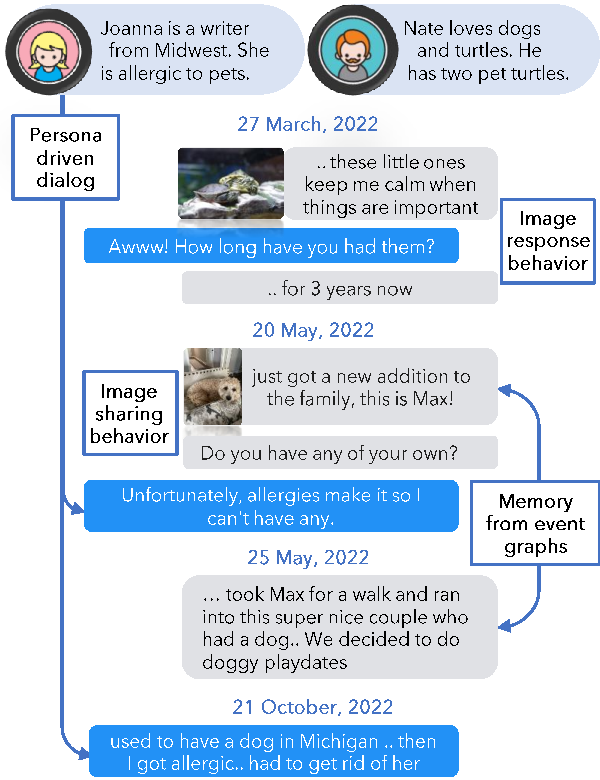
\includegraphics[width=0.48\textwidth]{figures/intro_figure_conv_only_v2.pdf}
    \caption{\textbf{An example in \dataset{}.} Dialogs are steered by the speakers' personas and corresponding events e.g., Joanna's responses are consistent with her pet allergies. For Nate, the event \textit{got a new dog} is followed by a \textit{playdate with neighbor's dog}, showcasing long-term memory. Multimodal dialog is enabled with image-sharing and image-response behaviors.
    }
    \label{fig:intro}
    \vspace{-15pt}
\end{figure}


\begin{table*}[t!]
\addtolength{\tabcolsep}{-4pt}
	\centering
	% \small
	\resizebox{0.99\textwidth}{!}{
		\begin{tabular}{p{2.7in}P{0.7in}P{0.9in}P{0.9in}P{1.2in}P{0.7in}P{2.0in}}
            \toprule
            \textbf{Dataset} & \textbf{Avg. turns per conv.} & \textbf{Avg. sessions per conv.} & \textbf{Avg. tokens per conv.} & \textbf{Time Interval} & \textbf{Multimodal} &  \textbf{Collection} \\
            \midrule
            MPChat \cite{ahn2023mpchat} & 2.8 & 1 & 53.3 & - & \ding{51} & Reddit \\
            MMDialog \cite{feng2023mmdialog} & 4.6 & 1 & 72.5 & - & \ding{51} & Social media\\
            Daily Dialog \cite{li2017dailydialog} & 7.9 & 1 & 114.7 & - & \ding{55} & Crowdsourcing \\
            SODA \cite{kim-etal-2023-soda} & 7.6 & 1 & 122.4 & - & \ding{55} & LLM-generated \\
            MSC \cite{xu2022beyond} (train; 1-4 sessions) & 53.3 & 4 & 1,225.9 & few days & \ding{55} & Crowdsourcing \\
            Conversation Chronicles \cite{jang2023conversation} & 58.5 & 5 & 1,054.7 & few hours - years & \ding{55} & LLM-generated \\
            \textbf{\dataset{} (ours)} & 304.9 & 19.3 & 9,209.2 & few months & \ding{51} & LLM-gen. + crowdsourc. \\           
            \bottomrule
        \end{tabular}
	}
        \vspace{-5pt}
        \caption{\textbf{Statistics of \dataset{}} compared to existing dialog datasets. The average length of a conversation in \dataset{} is 9x that of MSC \cite{xu2022beyond}, distributed over 6x more turns and 4x more sessions (on average).}
	\label{tab:compare_datasets}
\end{table*}


\begin{figure*}[t]
    \centering
    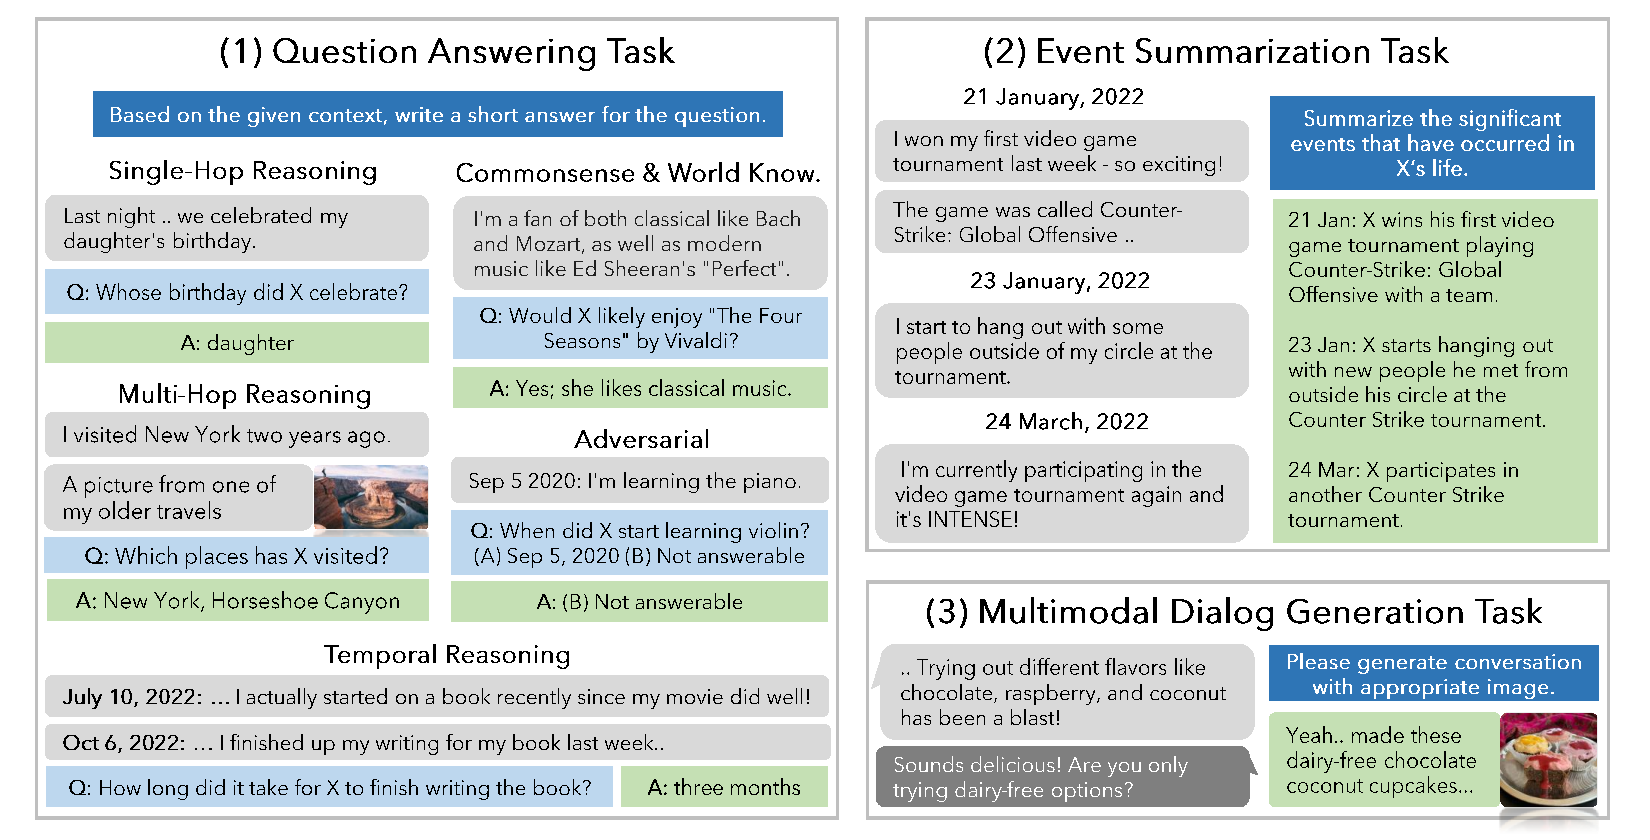
\includegraphics[width=\textwidth]{figures/evaluation_framework.pdf}
    \vspace{-20pt}
    \caption{\textbf{Overview of our evaluation framework}. We propose three tasks: question answering, event summarization and multimodal dialog generation to evaluate models' comprehension in very long-term dialogues.}
    \label{fig:eval-framework}
    \vspace{-1pt}
\end{figure*}


Despite recent advancements in dialogue models based on LLMs for extended contexts~\cite{bertsch2024unlimiformer, xiao2023efficient}, as well as the integration of retrieval augmented generation (RAG) techniques~\cite{shuster2021retrieval, ram2023context, shi2023replug}, there is still a need for thorough evaluation of their efficacy in handling very long conversations. Indeed, studies in long-term open-domain dialogues have concentrated on assessing model responses within limited contexts e.g., $\sim$1K tokens over five chat sessions~\cite{xu2022beyond, jang2023conversation, zhang2023mind}. This long term evaluation is crucial for refining engaging chatbots capable of remembering key information from past interactions, to generate empathetic, consistent, and useful responses.



To this end, we present the first study of very long-term open-domain multi-modal dialogues, closely mirroring real-world online interactions, collected via a human-machine pipeline where we first use LLM-based generative agents to generate conversations and then ask human annotators to fix any long-term inconsistencies in the conversations.
Specifically, drawing on the understanding that real-world conversations are a complex blend of collective memories~\cite{assmann1995collective, hirst2008towards}, individual viewpoints~\cite{hirst2018collective}, external influences~\cite{hirst2012remembering}, and the unique persona of the speakers~\cite{pruitt2003personas, cooper1999inmates, zhou2020design, shum2019sketch}, we create \textit{very long-term} dialogues based on LLM agent with the following features:
(1) a unique persona (\Sref{ssec:dataset-persona});
(2) a timeline of causally interlinked events in their lives (\Sref{ssec:temporal-event}); and (3) \textit{reflect \& response} mechanism to respond based on dialogue history (like in ~\citet{park2023generative}) and \textit{image sharing \& image reaction} behavior which sends or reacts to images (\Sref{ssec:llm-agent}). Finally, human annotators fix long-range inconsistencies in dialogues, remove irrelevant images, and verify the grounding of dialogs to events (\Sref{ssec:manual-filter}). With this pipeline, we create \dataset{}, a dataset of 50 \textit{very long-term} dialogues, each consisting of 300 turns and 9K tokens on avg., over up to 35 sessions (see Figure~\ref{fig:intro} and  Table~\ref{tab:compare_datasets}).  


Conventional approaches for evaluating conversational agents in open-domain dialogues involves directly evaluating the agent response based on past dialogue history.
It often employs lexical overlap~\cite{papineni-etal-2002-bleu} and semantic overlap~\cite{zhang2019bertscore} between ground truth and the agent response, or consistency~\cite{ghazarian2022deam}, contradiction~\cite{nie2021like, welleck2019dialogue}, and empathy~\cite{zhang2021dynaeval, zhang2022fined} of the agent response. However, these evaluation metrics are not well-suited for directly assessing the agent's comprehension of long-term contexts.

In this study, we present a holistic evaluation framework to assess an agent's proficiency in managing and responding within long-term contexts (see Figure~\ref{fig:eval-framework}). First, agents need to ``recall'' past context correctly to integrate relevant information into future responses. We present a direct examination of their \textit{memory} via a \textit{question answering} (QA) task (\Sref{ssec:benchmark-qa}). We classify questions into five distinct reasoning types to evaluate memory from multiple perspectives: single-hop, multi-hop, temporal, commonsense or world knowledge, and adversarial. Second, agents also need to recognize long-range causal and temporal connections in the dialogues to generate empathetic and relevant responses.
We propose a measurement of their causal and temporal understanding with an \textit{event graph summarization} task (\Sref{ssec:benchmark-event}). In this task, the event graphs linked to each LLM speaker serve as the correct answers, and models are tasked with extracting this information from the conversation history. Third, conversational agents need to utilize relevant context recalled from past conversations to generate responses that are consistent with the ongoing narrative. We assess this ability via the \textit{multi-modal dialog generation} task (\Sref{ssec:benchmark-mm}). 



We present extensive experimental results on the \dataset{} benchmark using instruction-based LLMs, long-context LLMs, and RAG techniques (\Sref{sec:baselines}). 
Our findings include:


(1) Long-context LLMs and RAG demonstrate effectiveness in QA tasks, improving `memory' capabilities of LLMs (with improvements ranging from 22-66\%), but still significantly lag behind human levels (by 56\%), especially in temporal reasoning, (by 73\%); 

(2) long-context LLMs demonstrate significant difficulty with adversarial questions in the QA task, showing a performance that is 83\% lower than the base model. They are especially prone to misassigning dialogs or events to the wrong speaker. 
Moreover, they show poor performance on \textit{event graph summarization}, lagging behind the base model by 14\%, indicating that they may grasp the factual elements within the entire conversation but do not accurately comprehend the context; and 

(3) RAG offers a balanced compromise, combining the accuracy of short-context LLMs with the extensive comprehension of wide-context LLMs, and does particularly well when dialogues are transformed into a database of assertions (\textit{observations}) about each speaker's life and persona.
